

\documentclass{beamer}

\mode<presentation> {

% The Beamer class comes with a number of default slide themes
% which change the colors and layouts of slides. Below this is a list
% of all the themes, uncomment each in turn to see what they look like.

%\usetheme{default}
%\usetheme{AnnArbor}
%\usetheme{Antibes}
%\usetheme{Bergen}
%\usetheme{Berkeley}
%\usetheme{Berlin}
%\usetheme{Boadilla}
%\usetheme{CambridgeUS}
%\usetheme{Copenhagen}
%\usetheme{Darmstadt}
%\usetheme{Dresden}
%\usetheme{Frankfurt}
%\usetheme{Goettingen}
%\usetheme{Hannover}
%\usetheme{Ilmenau}
%\usetheme{JuanLesPins}
%\usetheme{Luebeck}
%\usetheme{Madrid}
%\usetheme{Malmoe}
%\usetheme{Marburg}
%\usetheme{Montpellier}
%\usetheme{PaloAlto}
%\usetheme{Pittsburgh}
%\usetheme{Rochester}
%\usetheme{Singapore}
%\usetheme{Szeged}
%\usetheme{Warsaw}

% As well as themes, the Beamer class has a number of color themes
% for any slide theme. Uncomment each of these in turn to see how it
% changes the colors of your current slide theme.

%\usecolortheme{albatross}
%\usecolortheme{beaver}
%\usecolortheme{beetle}
%\usecolortheme{crane}
%\usecolortheme{dolphin}
%\usecolortheme{dove}
%\usecolortheme{fly}
%\usecolortheme{lily}
%\usecolortheme{orchid}
%\usecolortheme{rose}
%\usecolortheme{seagull}
%\usecolortheme{seahorse}
%\usecolortheme{whale}
\usecolortheme{wolverine}

%\setbeamertemplate{footline} % To remove the footer line in all slides uncomment this line
%\setbeamertemplate{footline}[page number] % To replace the footer line in all slides with a simple slide count uncomment this line

%\setbeamertemplate{navigation symbols}{} % To remove the navigation symbols from the bottom of all slides uncomment this line
}

\usepackage{graphicx} % Allows including images
\usepackage{booktabs} % Allows the use of \toprule, \midrule and \bottomrule in tables


\usepackage{listings}
\lstset{language=Java,
                basicstyle=\footnotesize\ttfamily,
                keywordstyle=\footnotesize\color{blue}\ttfamily,
}

%----------------------------------------------------------------------------------------
%	TITLE PAGE
%----------------------------------------------------------------------------------------

\title[Inheritance]{10.Inheritance} % The short title appears at the bottom of every slide, the full title is only on the title page

\author{Sakib Abrar} % Your name
\institute[BUET] % Your institution as it will appear on the bottom of every slide, may be shorthand to save space
{
CSE\\~\\Bangladesh University of Engineering \& Technology \\ % Your institution for the title page
\medskip
\textit{sakib.cghs@gmail.com} % Your email address
}
\date{\today} % Date, can be changed to a custom date

\begin{document}

\begin{frame}
\titlepage % Print the title page as the first slide
\end{frame}

\begin{frame}
\frametitle{Overview} % Table of contents slide, comment this block out to remove it
\tableofcontents % Throughout your presentation, if you choose to use \section{} and \subsection{} commands, these will automatically be printed on this slide as an overview of your presentation
\end{frame}

%----------------------------------------------------------------------------------------
%	PRESENTATION SLIDES
%----------------------------------------------------------------------------------------

%------------------------------------------------
\section{Inheritance Basics}
%------------------------------------------------

\begin{frame}
\frametitle{Inheritance Baciss}
\begin{itemize}
\item Inheritance can be defined as the process where one class acquires the properties (methods and fields) of another. With the use of inheritance the information is made manageable in a hierarchical order.
\item The class which inherits the properties of other is known as subclass (derived class, child class) and the class whose properties are inherited is known as superclass (base class, parent class).
\end{itemize}
\end{frame}


%------------------------------------------------

%------------------------------------------------
\section{DRY principle}
%------------------------------------------------

\begin{frame}
\frametitle{DRY : Don't Repeat Yourself}
\textbf{In coding try not to repeat yourself.}\\~\\
If you're getting a lot of similarities in two class then try to use inheritance.\\
This is like a parent child relationship.\\ Childs inherit some traits from their parent.\\
A Child class can inherit properties from parent class.
\end{frame}

%------------------------------------------------
\section{Java "extends" keyword}
%------------------------------------------------

\begin{frame}
\frametitle{Java "extends" keyword}
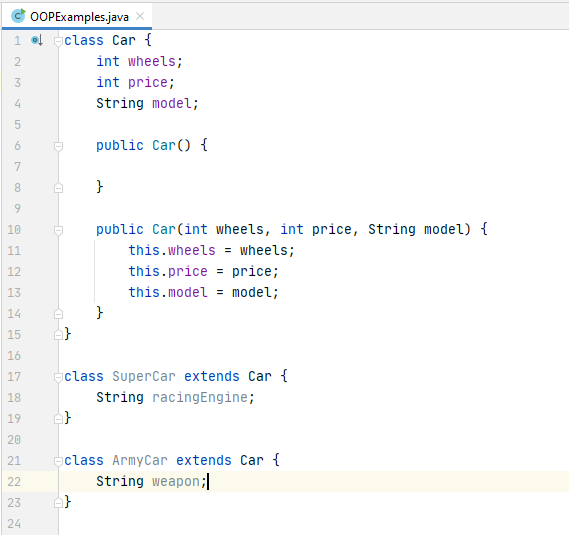
\includegraphics[width=0.8\textwidth]{BasicInheritance.png}
\end{frame}

%------------------------------------------------
\section{Java "super" keyword}
%------------------------------------------------

\begin{frame}
\frametitle{Java "super" keyword}
\textbf{You can use super to call parent class constructor in child class constructor.}\\~\\
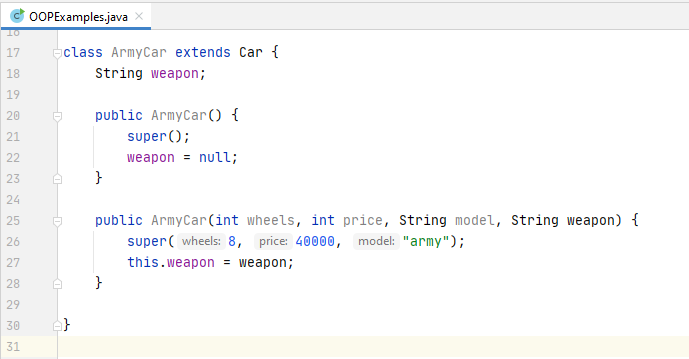
\includegraphics[width=\textwidth]{Super.png}
\end{frame}


%-----------------------------------------------
\section{Parent Class variable can hold child class data}
%-----------------------------------------------

\begin{frame}[fragile]{Parent Class variable can hold child class data}
\begin{columns}[T]
% code
\begin{column}{\textwidth}
\begin{lstlisting}
class Car {
    // Car data and methods
}

class SuperCar extends  Car {
    // SuperCar data and methods
}

class ArmyCar extends Car {
    // ArmyCar data and methods
}

public class InheritanceExamples {
    public static void main(String[] args) {
        Car amarGari = new ArmyCar();
        Car tomarGari = new SuperCar();
    }
}

\end{lstlisting}
\end{column}
% description
\end{columns}
\end{frame}


%------------------------------------------------


%------------------------------------------------

\begin{frame}[fragile]
\frametitle{Constructor Examples}
\textbf{You can also overload constructors:}
\begin{columns}[T]
% code
\begin{column}{\textwidth}
\begin{lstlisting}
class Car {
    int wheels;
    int price;
    String model;

    public Car(int wheels, int price, String model) {
        this.wheels = wheels;
        this.price = price;
        this.model = model;
    }

    public Car(int price, String model) {
        this.wheels = 4;
        this.price = price;
        this.model = model;
    }
}

\end{lstlisting}
\end{column}
% description
\end{columns}
\end{frame}

%------------------------------------------------


%-----------------------------------------------
\section{Default Constructor}
%------------------------------------------------

\begin{frame}
\frametitle{Default Constructor}
If you don’t implement any constructor in your class, the Java compiler inserts default constructor into your code on your behalf. \\You will not see the default constructor in your source code(the .java file) as it is inserted during compilation and present in the bytecode(.class file).\\~\\
The default constructor is inserted by compiler and has no code in it, on the other hand we can implement no-arg constructor in our class which looks like default constructor but we can provide any initialization code in it.
\end{frame}

%------------------------------------------------



%------------------------------------------------
\section{Access Modifiers in Java}
%------------------------------------------------

\begin{frame}
\frametitle{Access Modifiers}
\begin{itemize}
\item \textbf{Private:} The access level of a private modifier is only within the class. It cannot be accessed from outside the class.
\item \textbf{Default:} The access level of a default modifier is only within the package. It cannot be accessed from outside the package. If you do not specify any access level, it will be the default.
\item \textbf{Protected:} The access level of a protected modifier is within the package and outside the package through child class. If you do not make the child class, it cannot be accessed from outside the package.
\item \textbf{Public:} The access level of a public modifier is everywhere. It can be accessed from within the class, outside the class, within the package and outside the package.
\end{itemize}
\end{frame}


%------------------------------------------------

\begin{frame}
\frametitle{Understanding Java Access Modifiers}
\textbf{Let's understand the access modifiers in Java by a simple table:}\\~\\
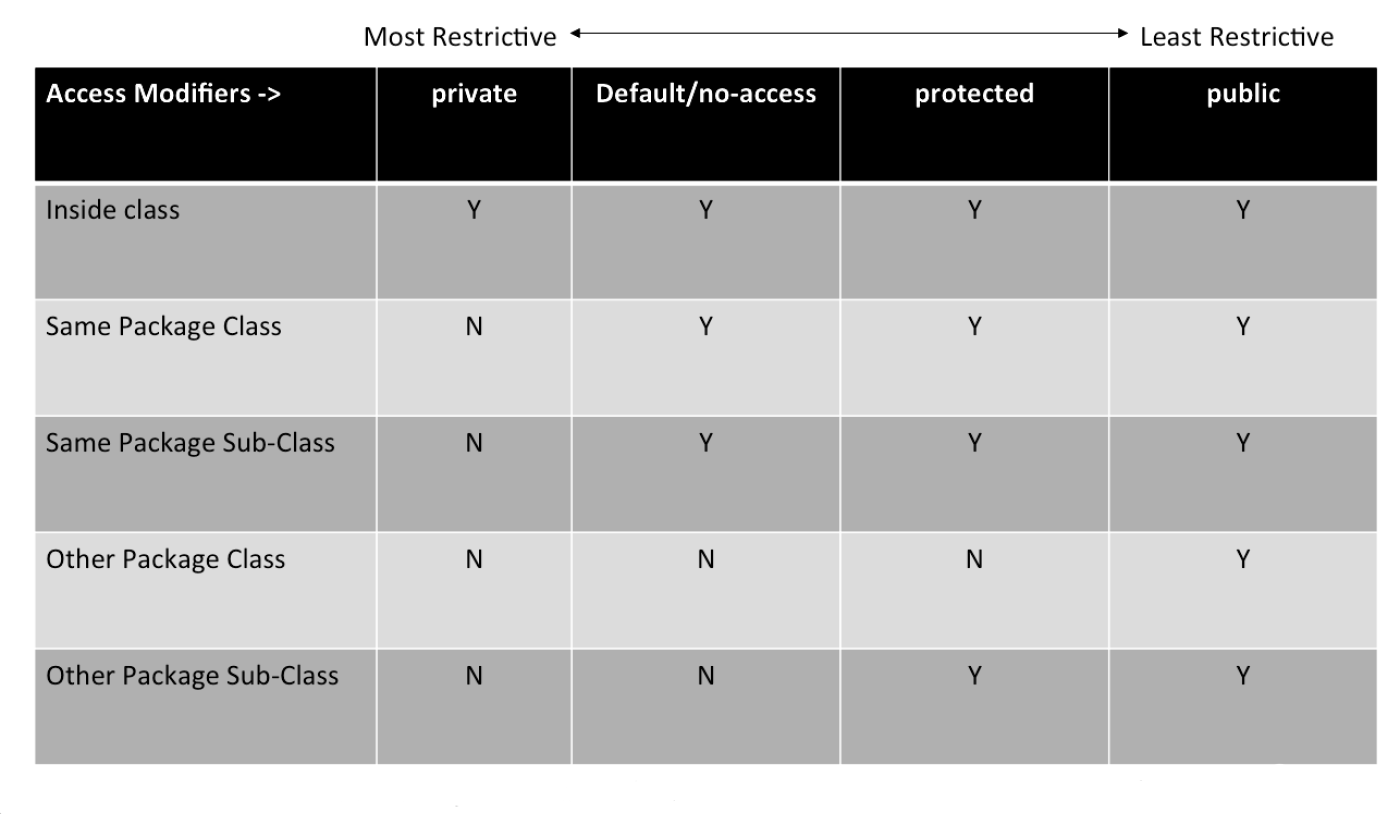
\includegraphics[width=\textwidth]{AccessModifier.png}
\end{frame}

%--------------------------------------------------

\begin{frame}
\Huge{\centerline{THE END }}
\end{frame}

%----------------------------------------------------------------------------------------

\end{document} 